\documentclass[a4paper,12pt]{article}
\usepackage[mag=1000]{newlistok}
\usepackage{tikz}
\usetikzlibrary{calc}

\УвеличитьШирину{1.3truecm}
\УвеличитьВысоту{2.2truecm}

\Заголовок{Отношение эквивалентности}
\НомерЛистка{22}
\renewcommand{\spacer}{\vfill}
\ДатаЛистка{12.09 -- 19.09/2018}
\Оценки{22/16/11}


\begin{document}

\СоздатьЗаголовок

\опр Пусть $X,Y$ --- множества. Множество упорядоченных пар
$ \{ (x,y) : x \in X, y \in Y \} $ называется {\em произведением множеств}
$X$ и $Y$. Обозначение $X \times Y.$
\копр

\задача Пусть в $X$ всего $n$ элементов, а в $Y$ --- $m$. Сколько элементов в $X \times Y$?
\кзадача

\задача Верно ли, что
\пункт $(A \times B) \cap (C \times D) = (A \cap C) \times (B \cap D) ;$
\пункт $(A \times B) \cup (C \times D) = (A \cup C) \times (B \cup D) ;$
\пункт $(A \times B)\setminus(C \times D) = (A \setminus C) \times (B \setminus D) ?$
\пункт Решите пункты а--в), если $B=D$.
\кзадача

% \опр Скажем, что на множестве $M$ задано (бинарное) отношение $R$,
% если для некоторых упорядоченных пар $(x,y)$  указано, что
% они {\em находятся в отношении} $R$. Обозначение $x\thicksim_Ry$.
% \копр

\опр {\em (Бинарным) отношением } на множестве  $M$ называется произвольное
подмножество $R$ в $M \times M.$ Если пара $(x,y)$ лежит в $R$, то мы говорим, что
$x$ находится в отношении $R$ с $y$. 
\\Обозначение: либо $xRy$, либо $x\thicksim_Ry$, либо просто $x\thicksim y$,
если понятно, о каком отношении идёт речь.
\копр

% \задача Докажите, что определения 2 и 3 эквивалентны.
% \кзадача

% {\em Пример:} если $G$ --- граф без петель и кратных рёбер, то $a\thicksim b \Leftrightarrow a\ \text{и}\ b\ \text{соединены ребром}$ --- бинарное отношение на множестве вершин графа $G$. Обратно, по всякому бинарному отношению можно построить граф, соединив $a$ и $b$ ребром тогда и только тогда, когда $a\thicksim b$.

\задача Сколько существует отношений на множестве из $n$ элементов?
\кзадача

\опр Отношение $\thicksim$ на множестве $M$ называется

1) {\em рефлексивным}, если $x\thicksim x$ для всех $x \in M;$

2) {\em симметричным}, если $x\thicksim y$ влечет $y\thicksim x$ для всех $x,y \in M;$

3) {\em транзитивным}, если $x \thicksim y$ и $y \thicksim z$ влечет $x \thicksim z$ для всех $x,y,z \in M;$

4) {\em отношением эквивалентности}, если оно и рефлексивно, и симметрично, и транзитивно.
\копр

\УстановитьГраницы{0cm}{3cm}
\задача
\righttikz{0mm}{0mm}{
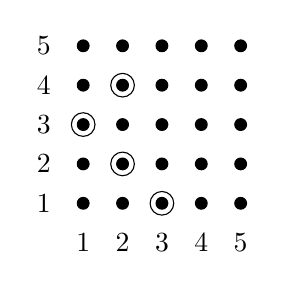
\begin{tikzpicture}[scale=0.5]
\foreach \x in {0,1,...,4} \foreach \y in {0,1,...,4} \node[draw,circle,inner sep=1.5pt,fill] at (\x,\y) {};
\foreach \x/\y in {1/1, 0/2, 2/0, 1/3} \draw (\x,\y) circle (0.3cm);
\foreach \y in {1,2,...,5} \draw (-1,-1)++(0, \y) node {\y};
\foreach \x in {1,2,...,5} \draw (-1,-1)++(\x, 0) node {\x};
\end{tikzpicture}}
На картинке справа изображено отношение $R$ на множестве $\hc{1,2,3,4,5}$,
состоящее из пар $\hc{(1,3), (2,2), (3,1), (2,4)}$.
Добавьте в него минимальное количество пар так, чтобы оно стало
\пункт рефлексивным;
\пункт симметричным;
\пункт транзитивным;
\пункт отношением эквивалентности;
\кзадача

\задача
\пункт Может ли отношение эквивалентности на множестве из 5 элементов состоять из 16 пар?
\пункт 17 пар?
\кзадача
\ВосстановитьГраницы

\ввзадача
\label{main}
Какие из следующих отношений рефлексивны, симметричны, транзитивны  и какие являются
отношениями эквивалентности?\\
\пункт
на множестве   натуральных чисел:
$x<y;$  $x \le y;$ $x$ делит $y;$ $x$ взаимно просто с $y$;\\ % $x$ и $y$ оканчиваются на одинаковую цифру;\\
\пункт
на множестве всех подмножеств натуральных чисел: $A \subset B$; $A \subseteq B$; \\
\пункт на множестве учеников 179 школы: $x$ и $y$ учатся в одном классе;\\
\пункт на множестве  графов с $n$ вершинами: $Г_1$ изоморфен $Г_2;$\\
\пункт на графе с $n$ вершинами: $x$ можно соединить ребром с $y$; $x$ можно соединить путем с $y$; $x$ и $y$ лежат в одной компоненте связности;\\
\ппункт[остатки от деления на $n$] на множестве целых чисел: $x\equiv y \bmod n$ для данного $n\in\N$;\\
\ппункт[целые числа] на множестве $\N\times\N$: $(a,b)\thicksim(c,d)$ если $a+d=b+c$;\\
\ппункт[рациональные числа] на множестве $\Z\times\N$: $(a,b)\thicksim(c,d)$ если $ad=bc$;\\
\ппункт[векторы] на множестве упорядоченных пар точек плоскости с действительными координатами: $((a,b),(c,d))\thicksim((e,f),(g,h))$ если $c-a=g-e$ и $d-b=h-f$.
\кзадача

% \задача Нарисуйте отношения эквивалентности из задачи 5а)
% для множества
% $Z_{15} =\{ 1,2,3,\dots,14\}$, $n = 1,2,3,4.$
% \кзадача

\опр Пусть на множестве $M$ задано отношение эквивалентности $\thicksim$. Для каждого элемента $a\in M$ {\em классом эквивалентности элемента $a$} называется
множество $H_а = \{ x \in M: x\thicksim a \}$.
\копр

\ввпзадача Докажите, что любые два класса эквивалентности либо не пересекаются, либо совпадают.
\кзадача

\опр Пусть на множестве $M$ задано отношение эквивалентности $\thicksim$. Множество классов эквивалентности называется {\em фактормножеством}
и обозначается $M/\thicksim$.
\копр


\ввзадача Опишите классы эквивалентности и фактормножество для отношений эквивалентности из задачи \ref{main} (письменно пункты е--и).
\кзадача

\опр
{\em Транзитивным замыканием} симметричного отношения $R$ на множестве $M$ называется отношение <<лежать в одной компоненте связности графа с вершинами из $M$ и рёбрами, соответствующими парам вершин, находящимся в отношении $R$>>.
\копр

\сзадача \пункт Докажите, что транзитивное замыкание симметричного отношения --- отношение эквивалентности.
\пункт Опишите транзитивные замыкания для отношений из задачи \ref{main}.
\пункт Опишите транзитивное замыкание для отношения $(a,b)\thicksim(b,a)$, $(a,b)\thicksim (a,b\pm a)$ на $\Z\times\Z.$
\кзадача


\сзадача
Сколько существует отношений эквивалентности на 8-элементном множестве?
\кзадача

\ЛичныйКондуит{0mm}{6mm}
% \GenXMLW


\end{document}

